%%%%%%%%%%%%%%%%%%%%%%%%%%%%%%%%%%%%%%%%%
% Dreuw & Deselaer's Poster
% LaTeX Template
% Version 1.0 (11/04/13)
%
% Created by:
% Philippe Dreuw and Thomas Deselaers
% http://www-i6.informatik.rwth-aachen.de/~dreuw/latexbeamerposter.php
%
% This template has been downloaded from:
% http://www.LaTeXTemplates.com
%
% License:
% CC BY-NC-SA 3.0 (http://creativecommons.org/licenses/by-nc-sa/3.0/)
%
%%%%%%%%%%%%%%%%%%%%%%%%%%%%%%%%%%%%%%%%%


%----------------------------------------------------------------------------------------
%	PACKAGES AND OTHER DOCUMENT CONFIGURATIONS
%----------------------------------------------------------------------------------------

\documentclass[final,hyperref={pdfpagelabels=false}]{beamer}

\usepackage[orientation=landscape]{beamerposter} % Use the beamerposter package 
%\usepackage[orientation=landscape,size=a2,scale=1.0]{beamerposter} % Use the beamerposter package for laying out the poster with a portrait orientation and an a0 paper size
\usepackage[utf8]{inputenc}
\usetheme{I6pd2} % Use the I6pd2 theme supplied with this template

\usepackage[english]{babel} % English language/hyphenation

\usepackage{amsmath,amsthm,amssymb,latexsym} % For including math equations, theorems, symbols, etc
\usepackage{natbib}

%\usepackage{times}\usefonttheme{professionalfonts}  % Uncomment to use Times as the main font
%\usefonttheme[onlymath]{serif} % Uncomment to use a Serif font within math environments

\boldmath % Use bold for everything within the math environment

\usepackage{booktabs} % Top and bottom rules for tables

\graphicspath{{fig/}} % Location of the graphics files

\usecaptiontemplate{\small\structure{\insertcaptionname~\insertcaptionnumber: }\insertcaption} % A fix for figure numbering
\usepackage[binary-units=true]{siunitx}
%\usepackage{formula}
%----------------------------------------------------------------------------------------
%	TITLE SECTION 
%----------------------------------------------------------------------------------------

\title{\huge Lunar images from the University of Stuttgart "Flying Laptop" satellite:
Scattered-light analysis.} % Poster title

\author{Jona Petri (1), Peter Thejll (2), Chris Flynn (3), Hans Gleisner (2), Sabine Klinkner (1), Sebastian Wenzel (1),
René Fléron (4), and Troelz Denver (4) } % Author(s)

	

\institute{(1) University of Stuttgart, Institute of Space Systems, Stuttgart, Germany, (2) Danish meteorological Institute, Lyngbyvej
100, DK-2100 Copenhagen Ø, Denmark, (3) Centre for Astrophysics and Supercomputing, Swinburne University of
Technology, Melbourne, Australia, (4) DTU Space, Danish Technical University, Lyngby, Denmark}


%----------------------------------------------------------------------------------------
%	FOOTER TEXT
%----------------------------------------------------------------------------------------

\newcommand{\leftfoot}{http://www.LaTeXTemplates.com} % Left footer text

\newcommand{\rightfoot}{pth@dmi.dk} % Right footer text

%----------------------------------------------------------------------------------------

\begin{document}

\addtobeamertemplate{block end}{}{\vspace*{2ex}} % White space under blocks

\begin{frame}[t] % The whole poster is enclosed in one beamer frame

\begin{columns}[t] % The whole poster consists of four major columns, each of which can be subdivided further with another \begin{columns} block - the [t] argument aligns each column's content to the top

\begin{column}{.01\textwidth}\end{column} % Empty spacer column

\begin{column}{.23\textwidth} % The first column

%----------------------------------------------------------------------------------------
%	OBJECTIVES
%----------------------------------------------------------------------------------------

\begin{block}{\huge{Abstract}}
\begin{itemize}
\item We study scattered-light properties of two telescopic systems, one on Earth and one in space, in order to determine the best systems approach for earthshine observing systems.
\item We explore the scattered-light properties of the University of Stuttgart "Flying Laptop" satellite.
\item We compare the properties of the scattered-light halo around the lunar disk as seen from the ground and from space.
\item We suggest improvements to earthshine observing techniques.
\end{itemize}
\end{block}

\begin{block}{The motivation}
Earthshine is the sunlight reflected from Earth striking the Moon and observed as reflected light. The \textbf{intensity of the earthshine is a measure of} the short-wave reflectivity, or albedo, of planet Earth, and is therefore an especially important quantity to measure in terms of the \textbf{climate change} debate.
 
Accurate, precise and long-duration observing campaigns of earthshine in these years of accelerating climate change \textbf{can become vital independent records} of the state of Earth, in decades to come.

Measurement of earthshine intensity faces all the problems of classical photometry: detection sensitivity stability is central --- without it, the accuracy of the observations is at stake. Precision (i.e. scatter) is important too, but fortunately, modern instrumentation has reached the level that averaging data is sufficient to beat random error down enough that climate-change studies can be performed.

\textbf{It is in the accuracy (lack of biases, and particularly, the absence of time-varying bias) that the core of the problem lies.}

\textbf{In this work} we explore the possibility that observing earthshine from outside the atmosphere, here with the University of Stuttgart Flying Laptop MICS camera, can be superior to traditional telescopic photometry from below the often cloudy and dynamically unstable atmospheric layer. One can imagine dedicated earthshine satellite instruments could be deployed to space, \textbf{provided the benefits and draw-backs of satellite optical instrumentation are fully understood}.

\end{block}


            
\begin{block}{The problem}
 
Earthshine is weak and has to be measured very close to a bright source of light --- the sun-lit side of the Moon --- so that cattered light becomes a particularly difficult problem. Under the atmosphere, the light scattered from the bright side of the Moon onto the earth-lit side, by the Mie scattering in the air, has to be removed at the data-reduction stage. Light is also scattered and diffracted by optics --- \textbf{how strong is typical atmospheric scattering} compared to optics-induced scattering? \textbf{Understanding that is the question of the present poster,} and our main tool for answering it is to compare images of the Moon obtained through the atmosphere, with images obtained  from space.
\end{block}

%----------------------------------------------------------------------------------------
%	INTRODUCTION
%----------------------------------------------------------------------------------------
\begin{block}{The MICS camera}
\begin{figure}
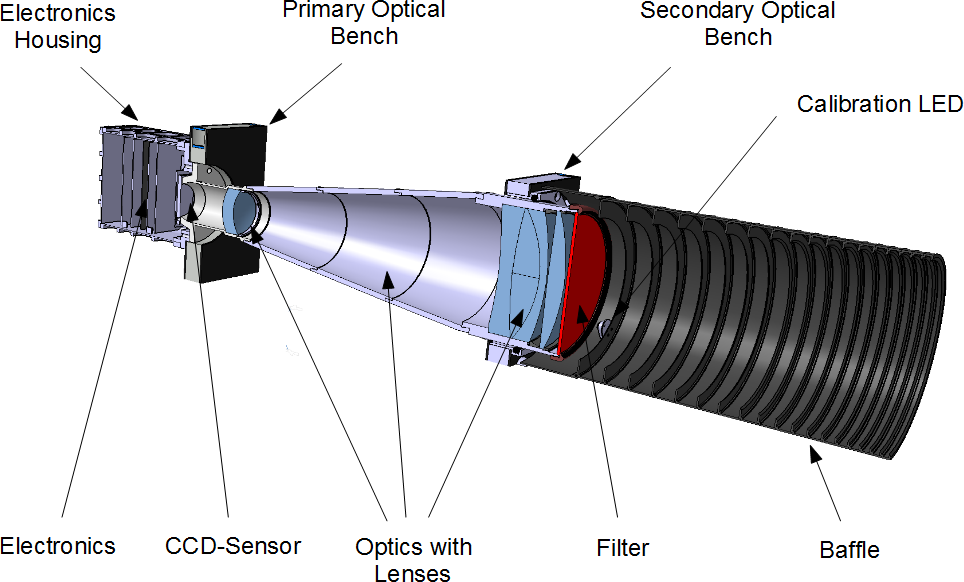
\includegraphics[scale=0.76]{fig/MICS_open_eng.png}
\caption{One of the MICS cameras. There is one such system for each of the colour filters.}~\label{fig:MICS}
\end{figure}
\end{block}

\end{column}

%----------------------------------------------------------------------------------------



\begin{column}{.01\textwidth}\end{column} % Empty spacer column
 
\begin{column}{.23\textwidth} % The second column


%----------------------------------------------------------------------------------------
%	MATERIALS
%----------------------------------------------------------------------------------------

\begin{block}{The satellite "Flying Laptop", and its MICS camera}
\begin{figure}
\includegraphics[scale=0.3]{fig/FLP_1_weiss.jpg}
\caption{The University of Stuttgart Flying Laptop satellite. The three optical instruments we use in this poster are seen at the upper left of the \SI[product-units = power]{60 x 70 x 87}{\centi\metre} body of the satellite.}~\label{fig:flp}
\end{figure}
The Flying Laptop (FLP) is a satellite developed by graduate and undergraduate students at the Institute of Space Systems of the University of Stuttgart with support by space industry and research institutions. The satellite weights about 110 kg and has a size of \SI[product-units = power]{60 x 70 x 87}{\centi\metre}. The main objective of its mission is earth observation, technology demonstration and education. Therefore, different payloads are used: The main one is the Multispectral Imaging Camera System (MICS), which consists of three identical cameras with different filters (see Image \ref{fig:MICS} and \ref{fig:filterfig}). Other payloads include a wide angle camera (PamCam) and an automatic identification system (AIS) receiver for observation of ships. The satellite was launched in July 2017 and is now used for earth observation and for student education. All operations are performed from the control room at the Institute of Space Systems and have been highly automated. The satellite bus has proven to be reliable and performs well. Besides the presented moon observation, the satellite also images the earth and observes ships using the AIS system. \\
Each camera in the MICS system has its own CCD detector, and each camera has its own main multi-element objective and baffle (located inside the satellite). The MICS has the following specifications:
\begin{itemize}
    \item Objective is a 5-element lens
    \begin{itemize}
        \item Aperture diameter ~\SI{90}{\milli\meter}
        \item focal length \SI{360}{\milli\metre}, f-number  4
    \end{itemize}
    \item Image sensor is a Kodak KAI-1003M CCD interline sensor 
    \begin{itemize}
        \item 12-bit dynamic range
        \item Bias-frames have a regular pattern. See Figure~\ref{fig:filterfig}
    \end{itemize}
    \item There are three broad-band interference filters for \SIrange{530}{580}{\nano\meter} (Green), \SIrange{620}{670}{\nano\meter} (Red), and \SIrange{820}{870}{\nano\meter} (NIR).(See Figure~\ref{fig:filterfig}).
\end{itemize}

\begin{figure}
    \centering
    \vspace{-1cm}
    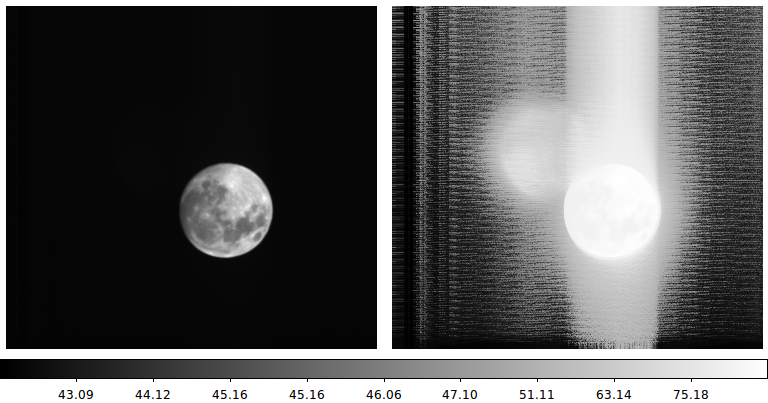
\includegraphics{fig/Moon2panels.png}
    %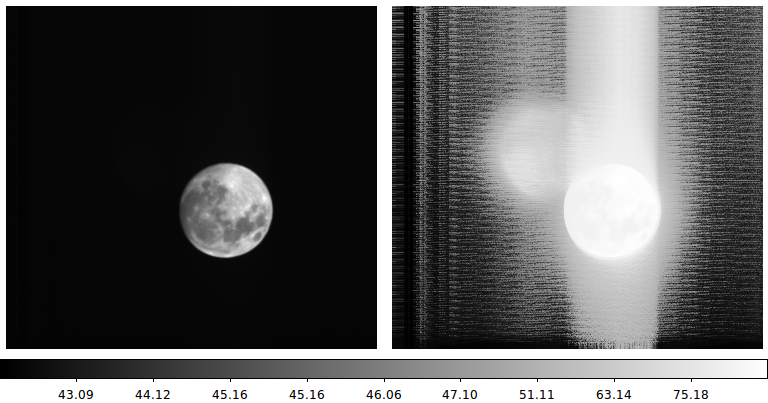
\includegraphics[viewport=10 47 750 310,clip]{fig/Moon2panels.png}
    \caption{MICS image of the Moon taken from orbit on February 18 2019, in the NIR filter band. The left panel shows the linear image while the right panel shows the histogram equalised image to bring  out the faint details. The features seen apart from the Moon itself are ghost images of the Moon caused by reflection from the CCD surface onto the back of the optical elements of the camera, and re-reflected several times. The vertical streak of light is due to illumination of the image sensor during image readout and occurs when the exposure time (here, \SI{8}{\milli\second}) is short compared to the readout time. The downward-pointing streak is puzzling.}
    \label{fig:my_label}
\end{figure}


\end{block}

\end{column} % End of the second column
\begin{column}{.01\textwidth}\end{column} % Empty spacer column

\begin{column}{.23\textwidth} % The third column
%---------------------------------
% PART 2
%---------------------------------
\begin{block}


\begin{figure}
    \centering
    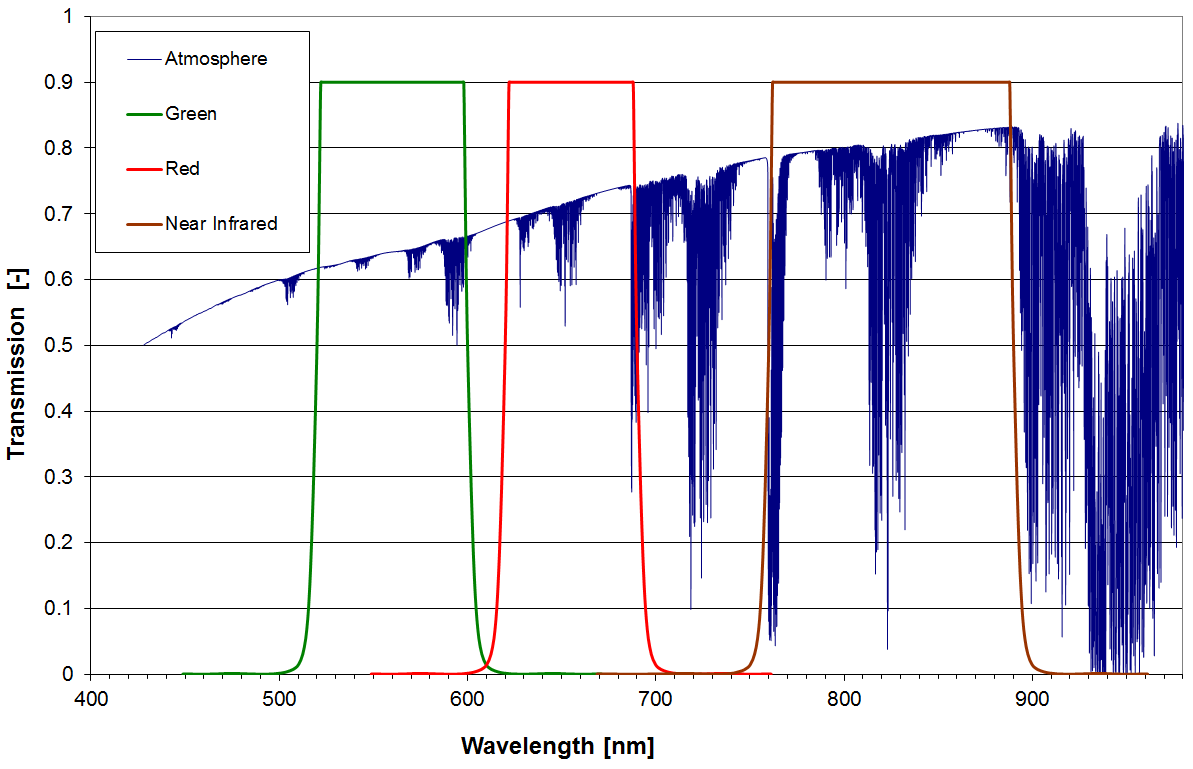
\includegraphics[scale=0.41]{fig/mics_filter_characteristics.png}
    \hspace{0.5cm}
    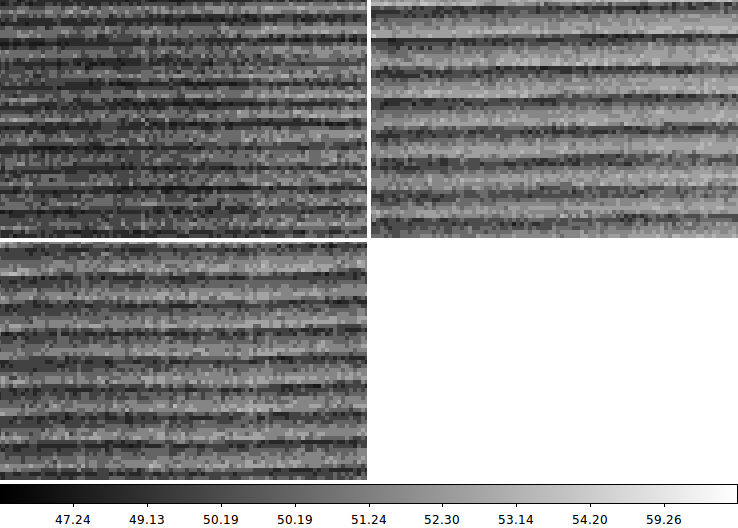
\includegraphics[scale=0.41]{fig/ripplefig.png}
    \caption{(Left panel): Transmission properties of the Green, Red and Near-Infrared (NIR) filters used in the three MICS cameras. Earth's atmospheric transmission spectrum is also shown, highlighting the absorption bands from CO$_2$ and H$_2$O.(Right panel): Structure of the dark frame in Red, Green and NIR (clockwise from upper left). Mean values near 50 counts, standard deviation about x counts. From 11 to 13 images in each of the three colour-bands have been aligned and averaged. Image scale and location in the image is the same for all three subpanels. }
    ~\label{fig:filterfig}
\end{figure}

\end{block}

\begin{block}{Expectations for point-spread function profiles.}
Diffraction in optics, and most optical defects (micro-scratches in lens surfaces, for instance) produce point-spread functions (PSFs) with power-law wings. Observing any object with such systems produces images with power-law profiles at intensity edges. In addition to this, scattering in the atmosphere also results in additional power-law behaviour in the resulting PSF. 

The end-result is different, however, if the object being observed is a point source (like a star), or a line (like a leaser-beam in a turbid atmosphere) or more extended objects such as semi-infinite planes or large illuminated disks (such as a full Moon).

An optical system produces diffraction patterns around objects viewed. In mono-chromatic light, the diffraction ripples of the Airy function are easily seen, but in broad-band light, such as with the MICS filters, the envelope of the diffraction pattern becomes that of a $1/r^3$ function.

Viewing objects with different geometries and extents with such a diffraction-PSF yields halos of scattered light around the edges of the object with profiles that depend on the geometry of the object and the distance from the edge.

For a range of geometries we find:
\begin{itemize}
    \item A point-source yields a $1/r^3$ profile for the intensity falloff with distance
    \item A line-source yields a $1/r^2$ profile with perpendicular distance from the line, $r$, and
    \item A semi-infinite half-plane yields a $1/r$ profile, while
    \item a uniform disk yields a variable dependence with $r$, similar to $1/r$ close to the edge and asymptotically approaching $1/r^3$ as the distance to the edge grows.
\end{itemize}

Any additional structure around an object, caused by light-scattering before the light arrives at the telescope objective --- scattering in  the atmosphere for instance, or by the main objective front surface (dust or scratches) --- would broaden the halo profile.

\textbf{We can therefore use the measured profile of halos around objects} observed by the MICS instrument to determine the dependency on distance from the object and \textbf{understand whether any additional source of light scattering} is present \textbf{beyond} that due to broad-band diffraction. 

\end{block}
%-----------------------------
% A model for return levels
%-----------------------------

\begin{block}{Halo profiles in space images.}

Figure~\ref{fig:3panelfig} shows the profile of the halo of the Full Moon images taken with the MICS from the night of February 16-17th and 18th 2019. Figure~\ref{fig:MLOresult} contains realistic estimates of the errors we expect in setting the level of the electronics-induced background in the images, and enables us to understand whether the profile significantly indicates a profile like a straight line (as expected from log-log plots of $1/r^{\alpha}$-type power laws) or not, in Figure~\ref{fig:3panelfig}.


%\vspace{-1cm}
%\end{block}

%\begin{block}
%\begin{figure}
%\centering 
%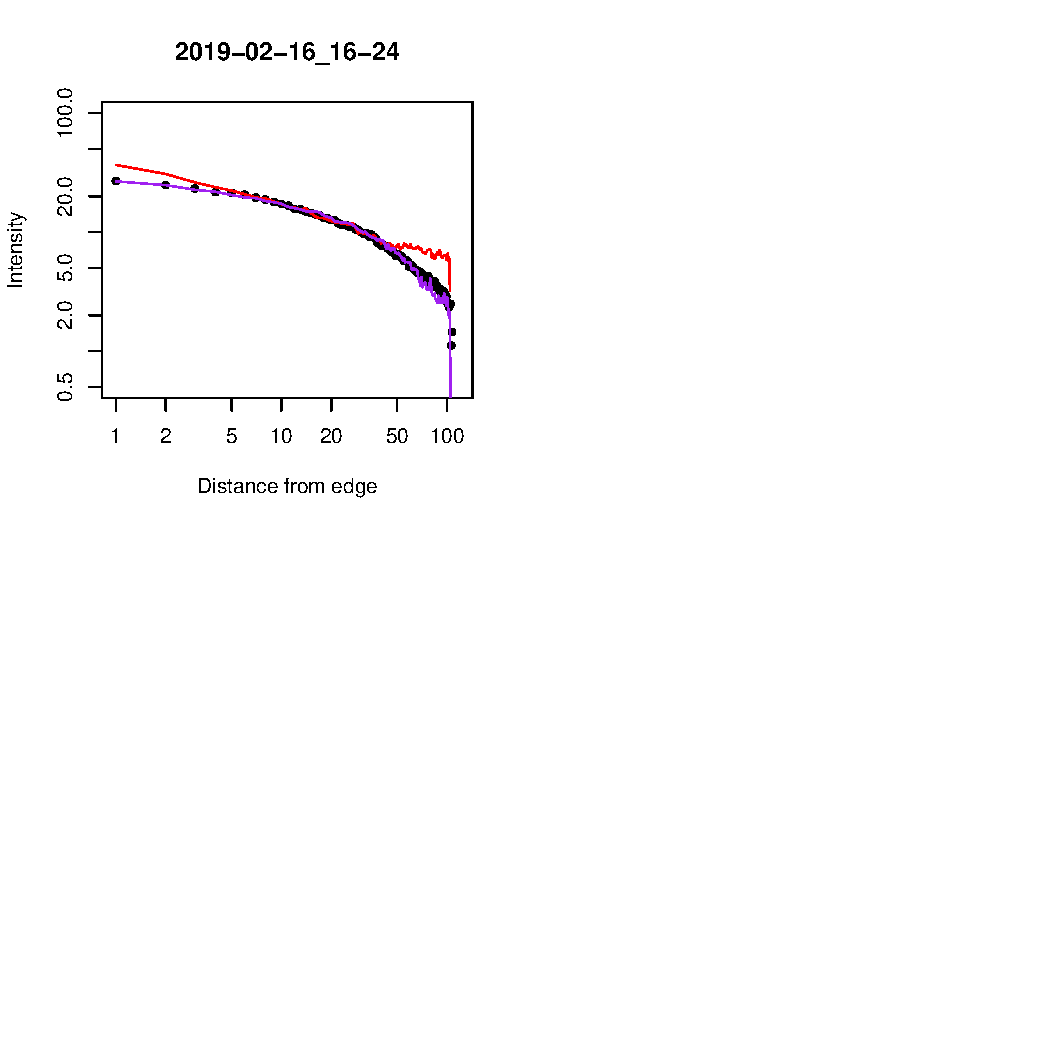
\includegraphics[scale=1.08,viewport=2 261 232 496,clip]{fig/slopes_compared_2019-02-16_16-24.pdf}
%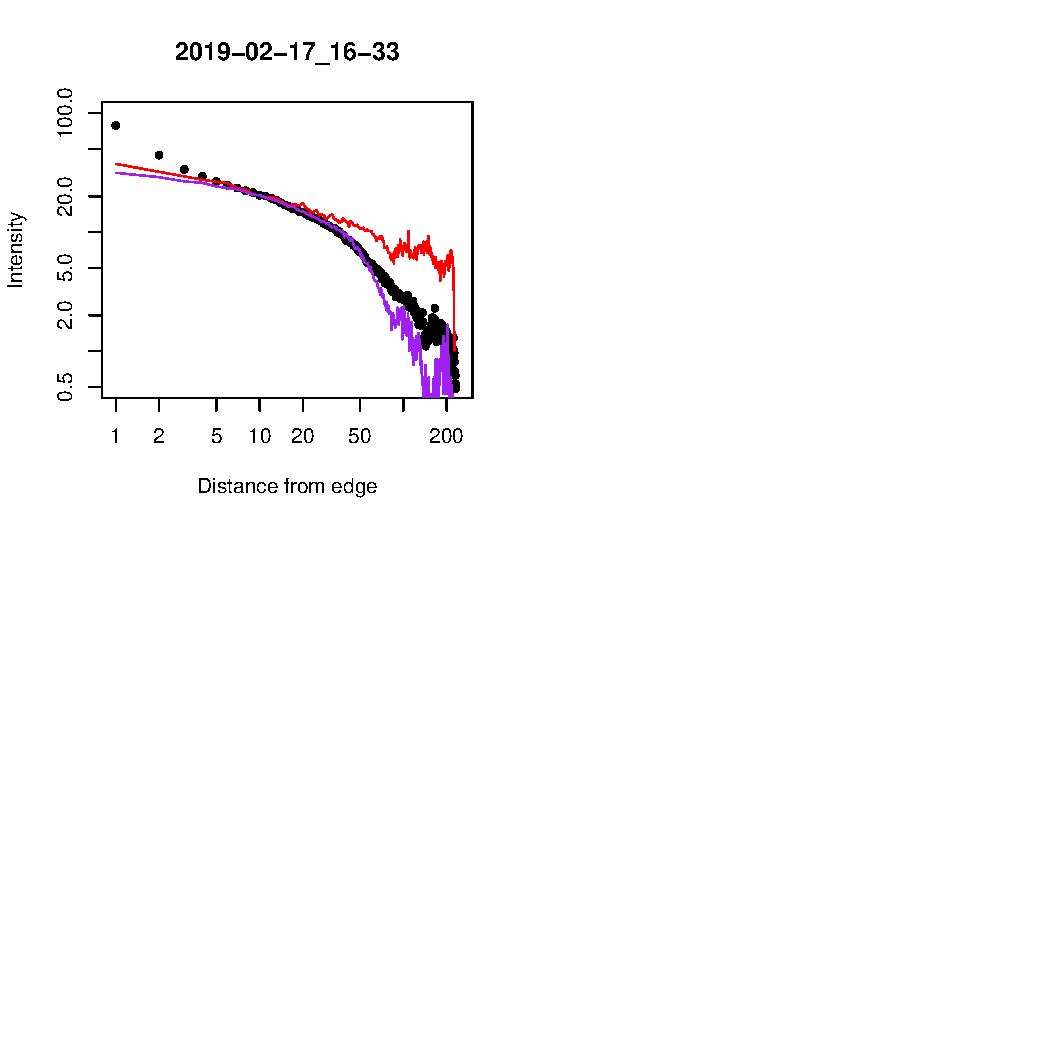
\includegraphics[scale=1.08,viewport=2 261 232 496,clip]{fig/slopes_compared_2019-02-17_16-33.pdf}
%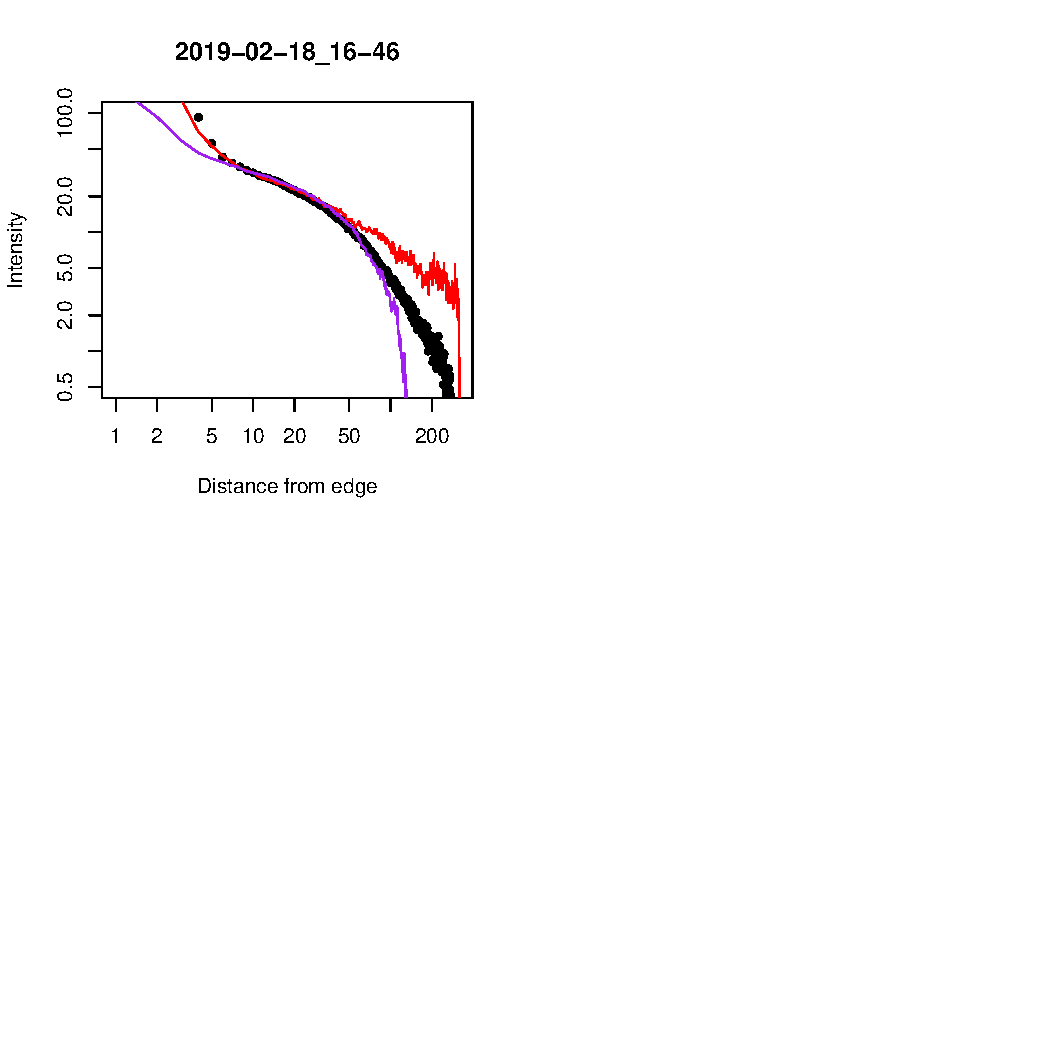
\includegraphics[scale=1.08,viewport=2 261 232 496,clip]{fig/slopes_compared_2019-02-18_16-46.pdf}
%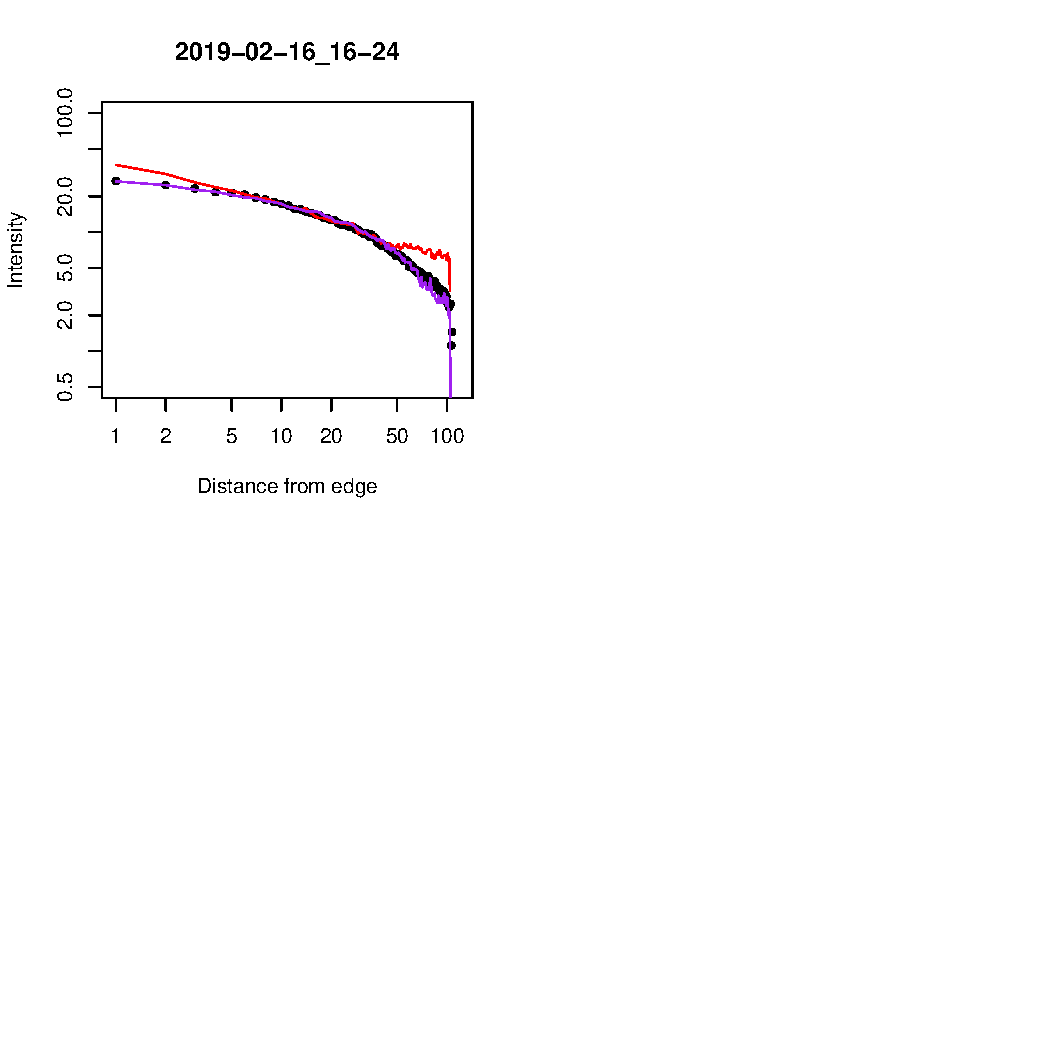
\includegraphics[scale=1.08,clip]{fig/slopes_compared_2019-02-16_16-24.pdf}
%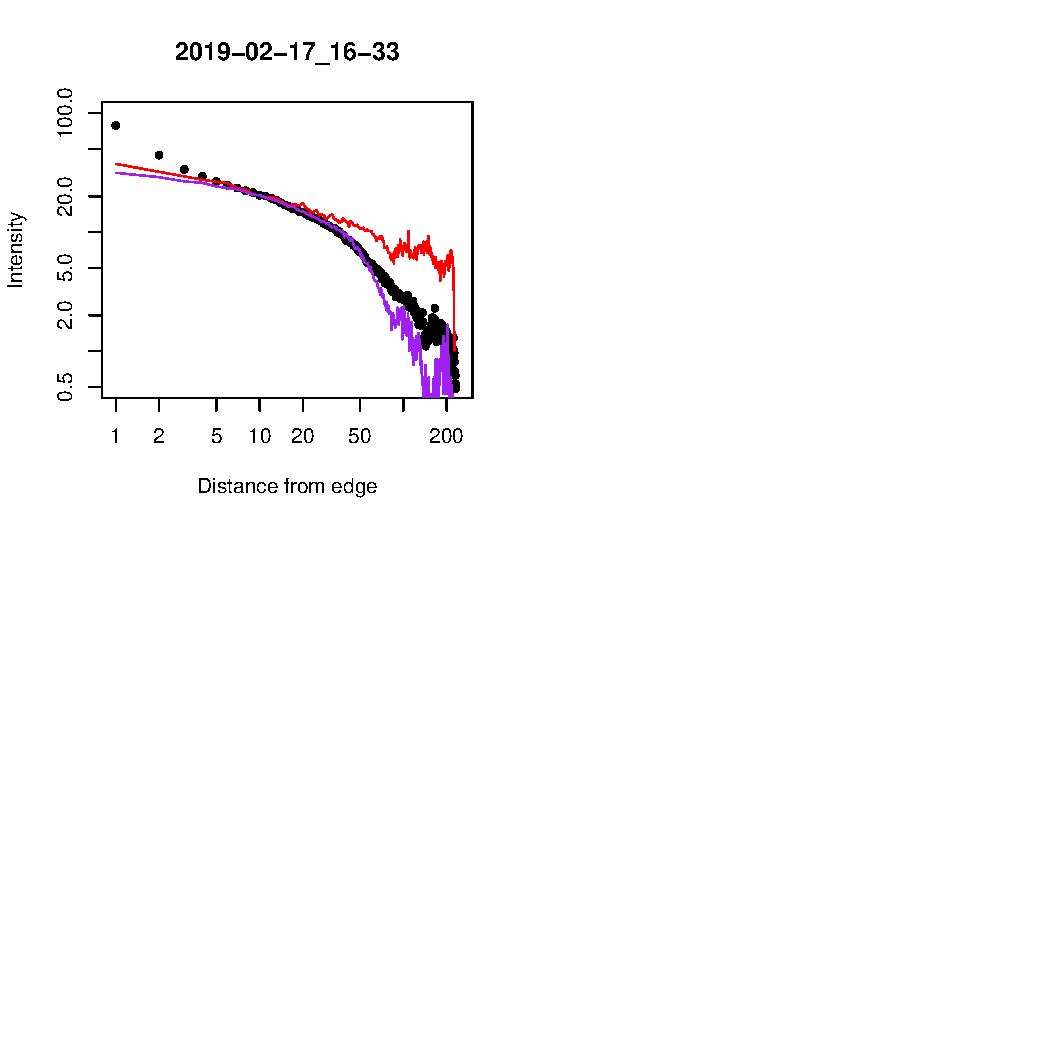
\includegraphics[scale=1.08,clip]{fig/slopes_compared_2019-02-17_16-33.pdf}
%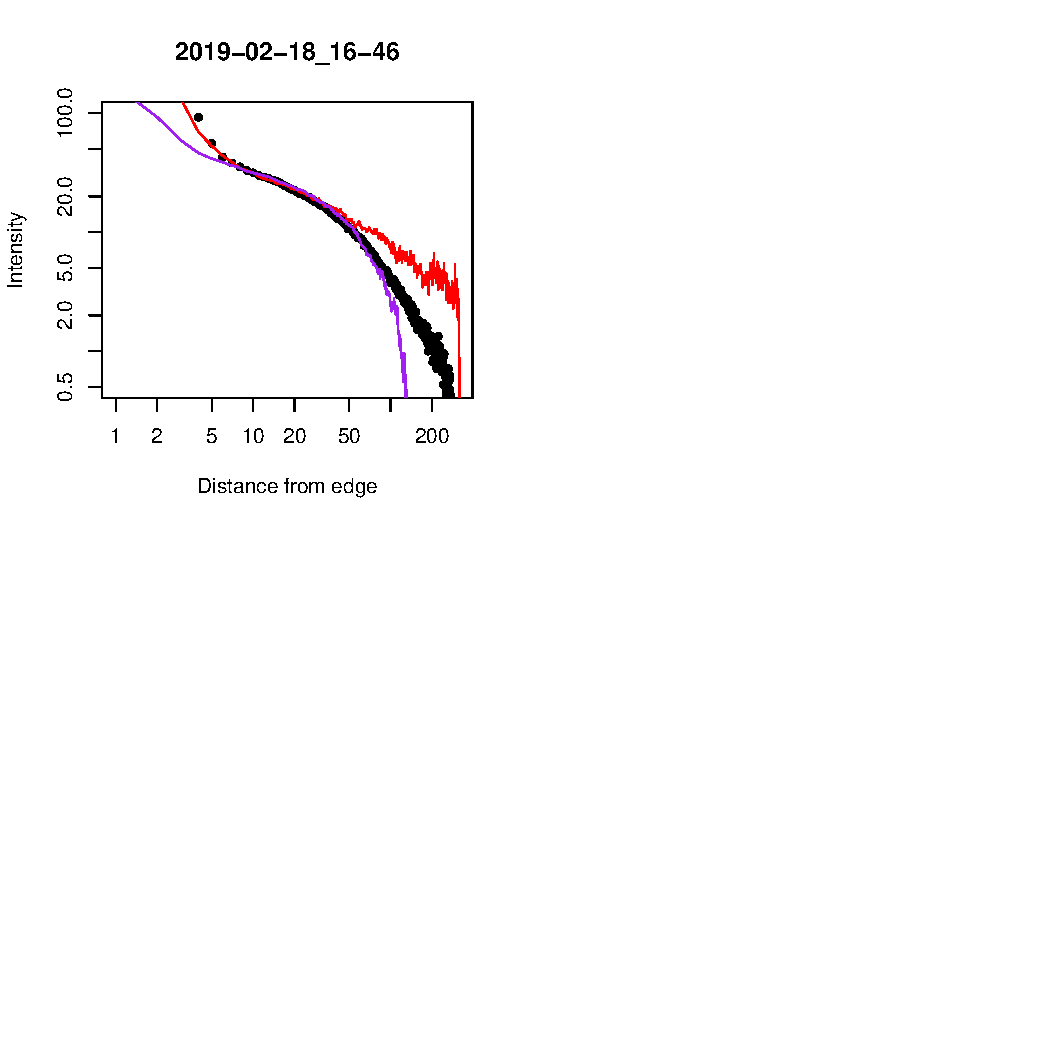
\includegraphics[scale=1.08,clip]{fig/slopes_compared_2019-02-18_16-46.pdf}
%\caption{Scattered-light halo profiles. The radial profile of the scattered light halo seen around the Full Moon disk on the nights of February 16th to 18th of 2019 were measured, in three colour bands, and are here plotted as function of the distance from the lunar disk edge. Black is the Green-filter profile, red is for a red filter, and purple is for a near-infrared filter. The intensities have been scaled to coincide at $r=10$.}~\label{fig:3panelfig}
%\end{figure}
\end{block}



\end{column} % End of the third column

\begin{column}{.01\textwidth}\end{column} % Empty spacer column
%----------------------------------------------------------------------------------------
\begin{column}{.23\textwidth}
%----------------------------------------------------------------------------------------
%	RESULTS
%---------------------------------------------------------------------------------------
\begin{block}{}
\begin{figure}
   \centering 
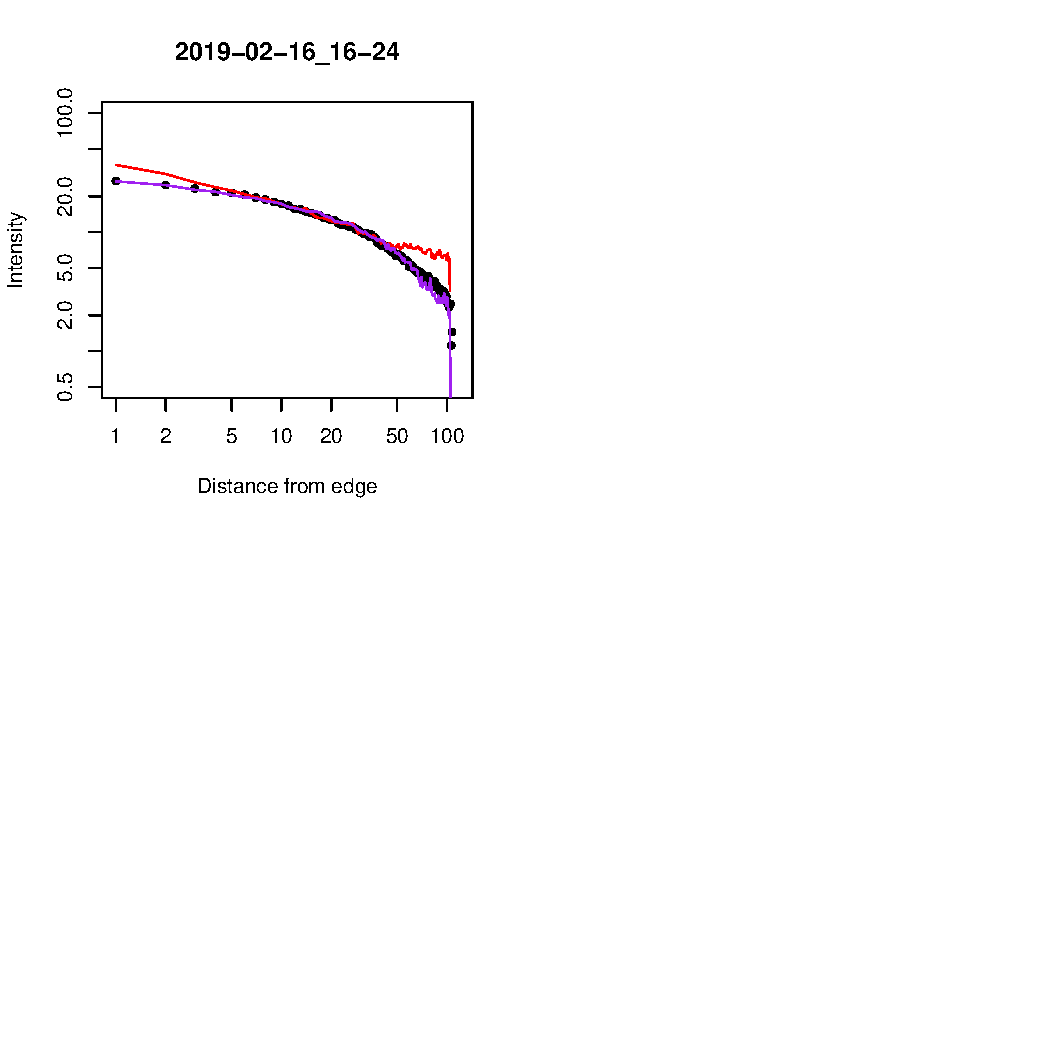
\includegraphics[scale=1.08,viewport=2 261 232 496,clip]{fig/slopes_compared_2019-02-16_16-24.pdf}
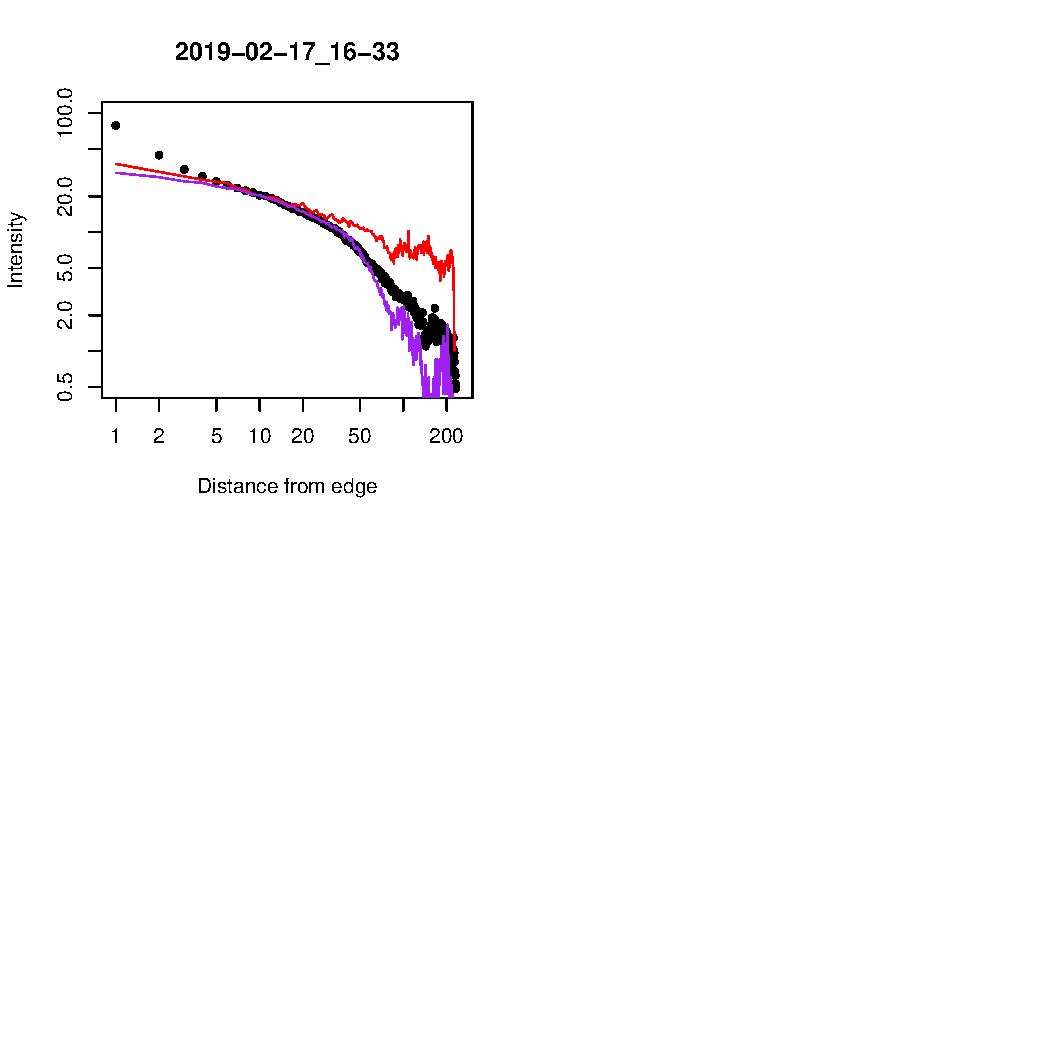
\includegraphics[scale=1.08,viewport=2 261 232 496,clip]{fig/slopes_compared_2019-02-17_16-33.pdf}
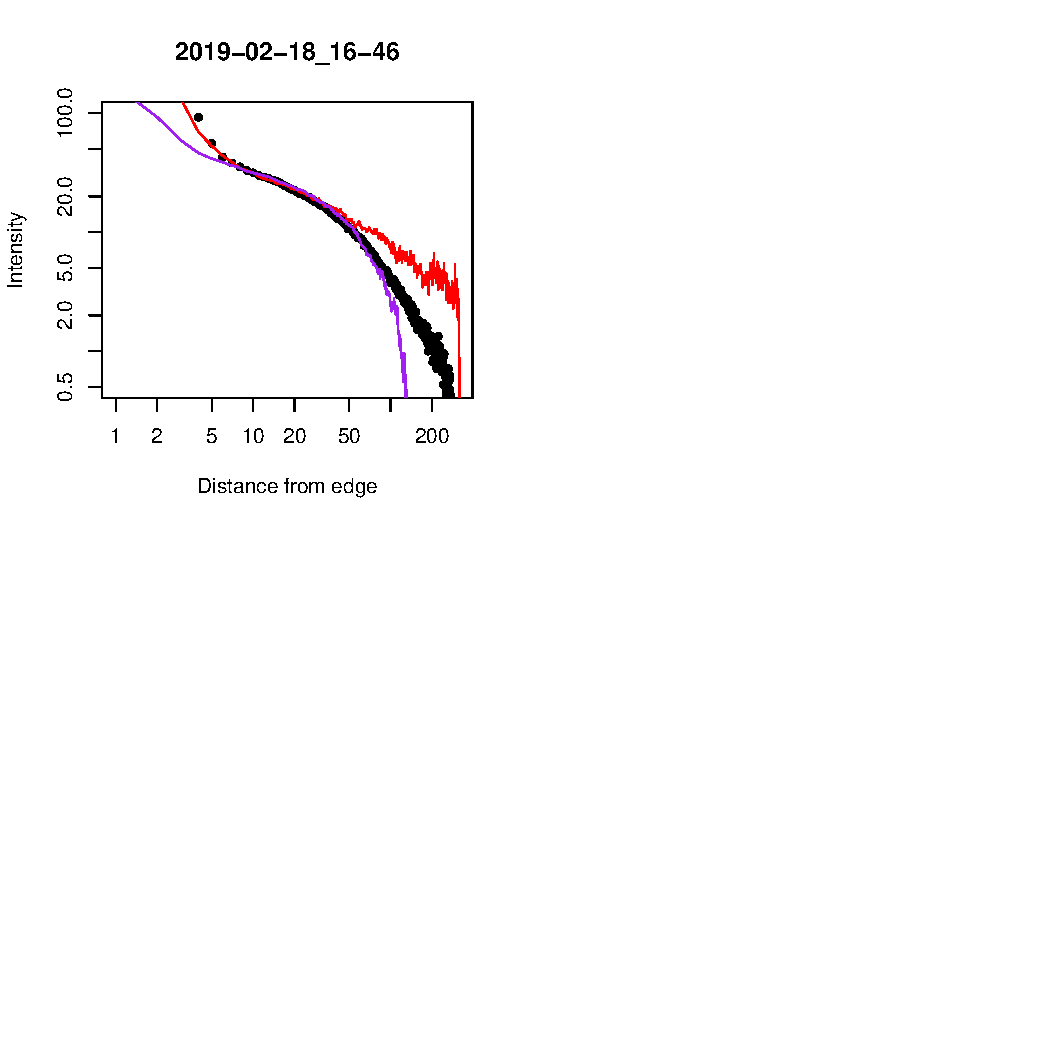
\includegraphics[scale=1.08,viewport=2 261 232 496,clip]{fig/slopes_compared_2019-02-18_16-46.pdf}
%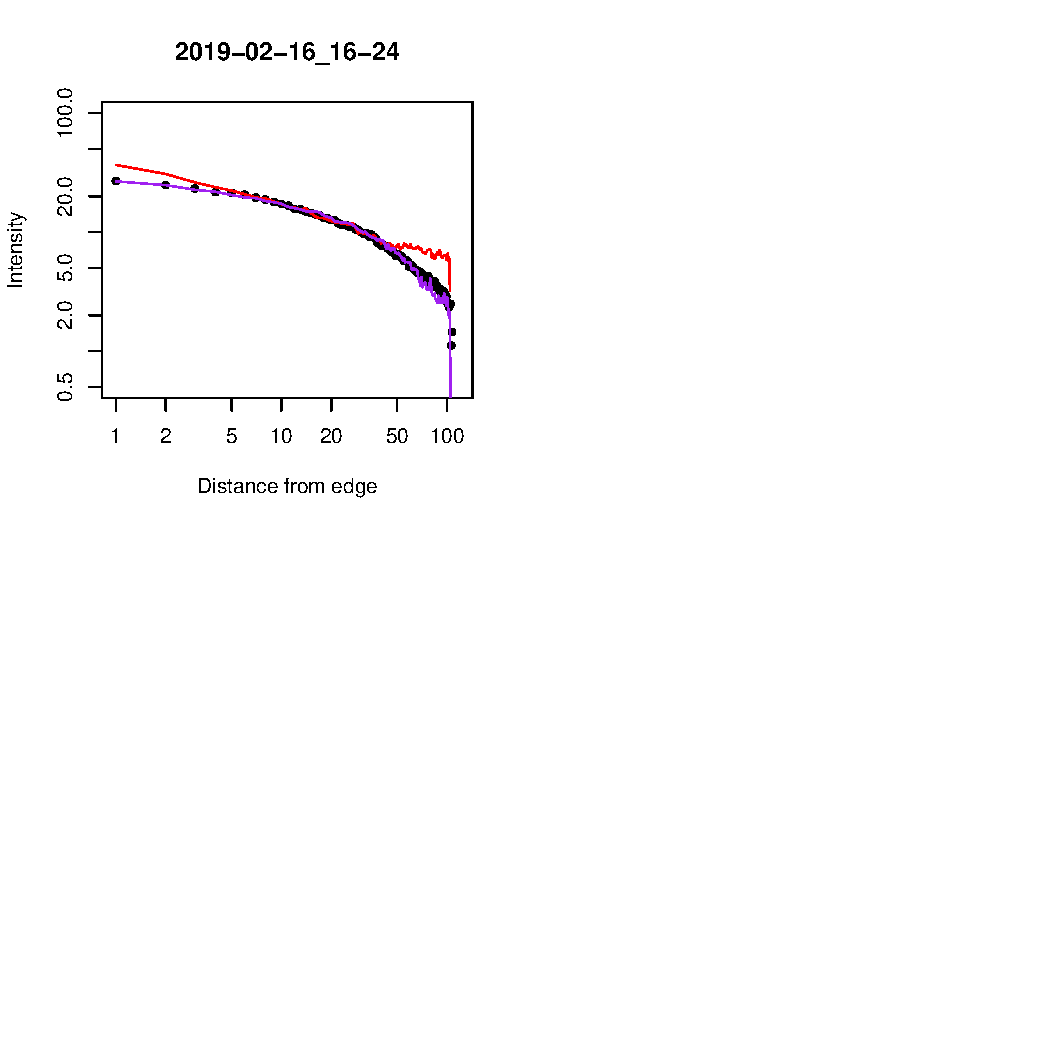
\includegraphics[scale=1.08,clip]{fig/slopes_compared_2019-02-16_16-24.pdf}
%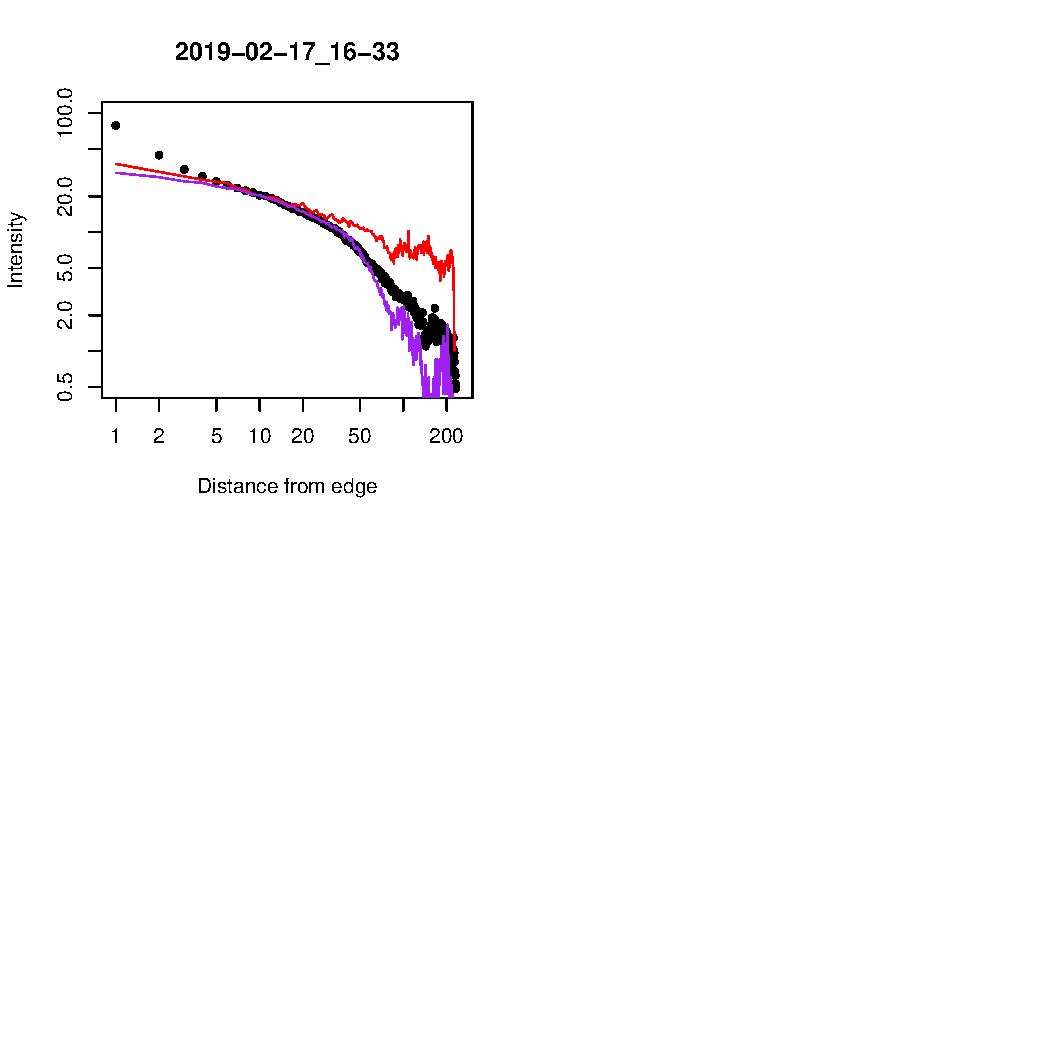
\includegraphics[scale=1.08,clip]{fig/slopes_compared_2019-02-17_16-33.pdf}
%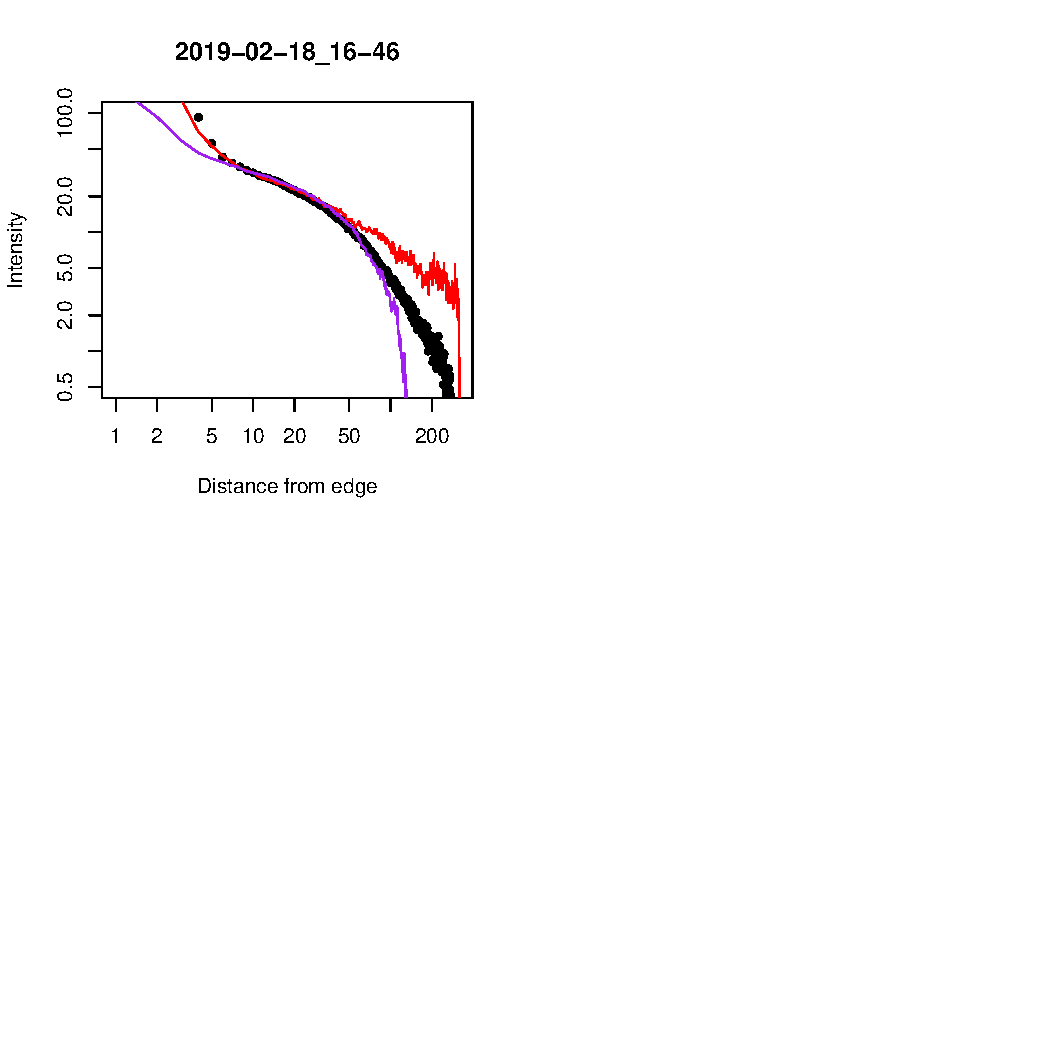
\includegraphics[scale=1.08,clip]{fig/slopes_compared_2019-02-18_16-46.pdf}
\caption{Scattered-light halo profiles. The radial profile of the scattered light halo seen around the Full Moon disk on the nights of February 16th to 18th of 2019 were measured, in three colour bands, and are here plotted as function of the distance from the lunar disk edge. Black is the Green-filter profile, red is for a red filter, and purple is for a near-infrared filter. The intensities have been scaled to coincide at $r=10$.}~\label{fig:3panelfig}
\end{figure}
\end{block}

\begin{block}{MICS Results for three colours}
\begin{table}[]
    \centering
    \begin{tabular}{ccc}
    Red & NIR & Green \\
    \hline
         --0.63 & --0.52 & --0.66\\
         \hline
    \end{tabular}
    \caption{Slopes of halo profiles in three colour bands, from log-log plots as in Figure~\ref{fig:3panelfig}. In each, the slope is estimated in the pixel range, counting from the lunar disk edge, 10 to 30 pixels.}
    \label{tab:my_label}
\end{table}
\end{block}
\begin{block}{Halo profile from a telescope on Earth compared to one from space}
\begin{figure}
\centering 
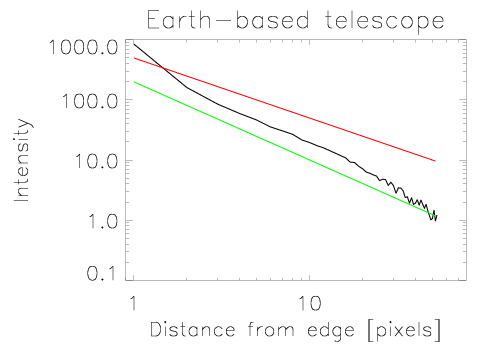
\includegraphics[scale=.7]{fig/MLOprofile.png}
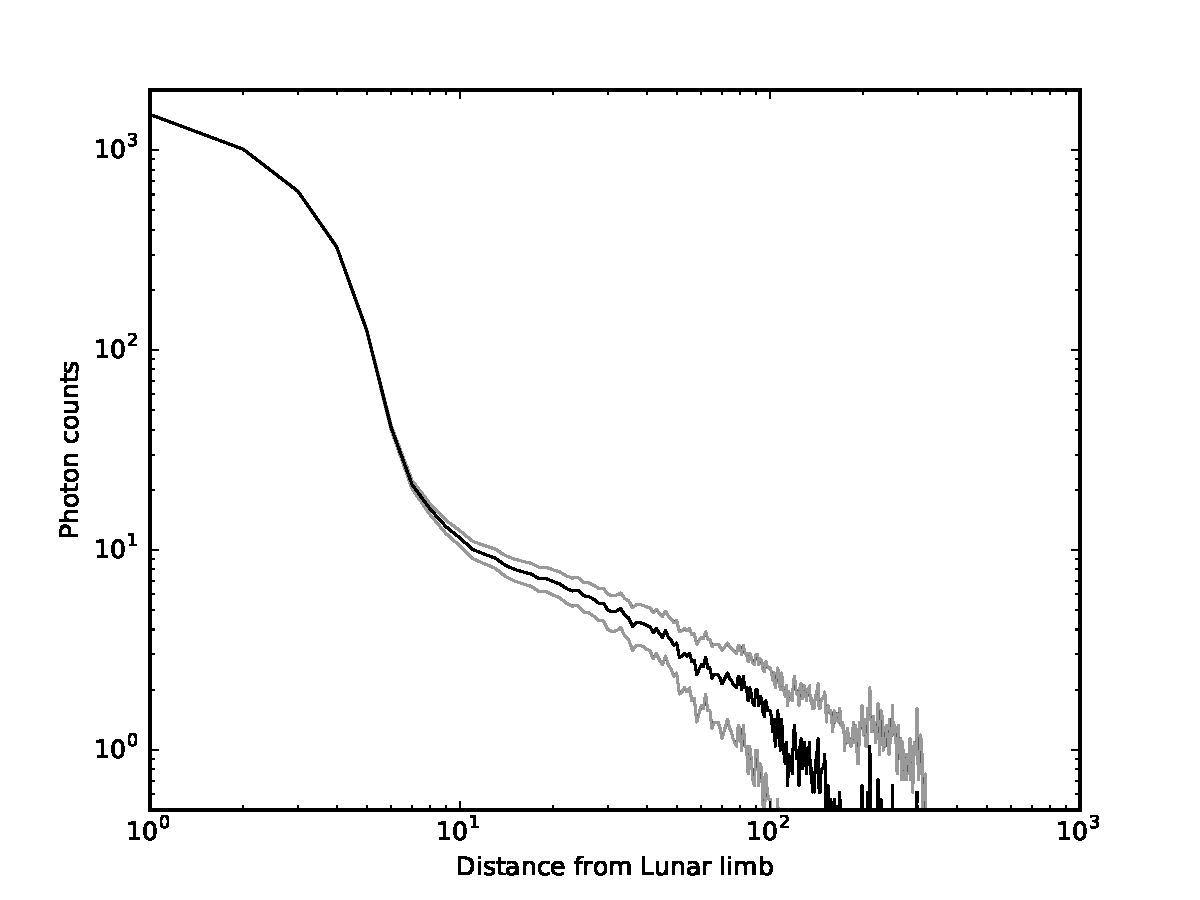
\includegraphics[scale=.6]{fig/fl-moon.pdf}
\caption{ (Left panel:) Scattered-light halo around the Moon as observed from Mauna Loa. Intensity is plotted as distance from the lunar edge. The Green line shows the slope of a $1/r^{1.3}$ power-law, while the red line is for a $1/r$ law. Near an illuminated disk theory predicts a diffraction-induced slope near 1. (Right panel:) Halo profile from MICS images (black line) and estimates of the uncertainty (grey), based on $\pm$ 1 sigma error on subtraction of the background for the Moon. The slope in the linear part is -0.52. }~\label{fig:MLOresult}
\end{figure}

\end{block}
\begin{block}{Summary}
\begin{itemize}
    \item We have measured the falloff of light beyond the lunar edge (the ``halo-slope'') of images of the Moon from the ground and from space.
    \item We find a shallow slope in the space-based images.
    \item The slope we find in the earth-based images suggest closer performance to what theory predicts for a diffraction-limited instrument observing through broad bands.
    \item The origin of the shallow slope in the images from space is unclear, but could be due to 'Ghost images' easily formed in a short focal-length instrument.
\end{itemize}

\end{block}

\begin{block}{Recommendations}
For a space-based imaging instrument to provide data comparable or superior to the current generation of Earth-based earthshine instruments the presence of ghost images caused by internal reflections in the camera system must be avoided.

Ghosting can be avoided by tilting the CCD axis,
    but small f-number systems do not allow tilted CCDs because of short focus depth.

%We therefore recommend the following:
%\begin{itemize}
    %\item A 16-bit image sensor is needed
    %\item Very low bias level --- a.k.a. readout noise, or RON, is required
    %\item A physical shutter --- or a "Global Shutter" (defined in electronics) --- preventing illumination of the sensor during readout, is required for short exposure times, such as these of the bright Moon.
    %\item Imaging without a coronograph optical design does not reduce stray light or diffraction from the aperture enough. A Lyot stop in the collimated part of the beam prior to third lens and image formation on the sensor is recommended.
%   \item A space-based earthshine instrument should have a relatively large f-number so that ghost elimination becomes possible by tilting the CCD axis away from the optical axis.
%\end{itemize}



\end{block}
 
%----------------------------------------------------------------------------------------
%	CONCLUSION
%----------------------------------------------------------------------------------------



%----------------------------------------------------------------------------------------
%	REFERENCES
%----------------------------------------------------------------------------------------

\begin{block}{References}
        
%\nocite{*} % Insert publications even if they are not cited in the poster
\small{\bibliographystyle{unsrt}
\bibliography{references}} 

\end{block}

%----------------------------------------------------------------------------------------
%	ACKNOWLEDGEMENTS
%----------------------------------------------------------------------------------------

\begin{block}{Acknowledgments}
\begin{itemize}
\small 
\item We thank...
\end{itemize}
\end{block}

%----------------------------------------------------------------------------------------
%	CONTACT INFORMATION
%----------------------------------------------------------------------------------------

\setbeamercolor{block title}{fg=black,bg=orange!70} % Change the block title color

%\begin{block}{Contact Information}
%\begin{itemize}
%\item Web: \href{http://www.dmi.dk}{www.dmi.dk} Email: \href{mailto:pth@dmi.dk}{PTH@dmi.dk} Phone: %+45 39 15 74 77
%\end{itemize}
%\end{block}



\end{column} % End of 4th column


\end{columns} % End of all the columns in the poster

\end{frame} % End of the enclosing frame

\end{document}
